\ifdefined\pdfinfoomitdate\pdfinfoomitdate=1\fi
\ifdefined\pdftrailerid\pdftrailerid{}\fi
\ifdefined\pdfsuppressptexinfo\pdfsuppressptexinfo=15\fi
\documentclass[conference]{IEEEtran}
\IEEEoverridecommandlockouts
\usepackage{cite}
\usepackage{amsmath,amssymb,amsfonts}
\usepackage{graphicx}
\usepackage{textcomp}
\usepackage{xcolor}
\usepackage{booktabs}
\usepackage{array}
\usepackage{placeins}
\usepackage{flushend}
\usepackage[hidelinks]{hyperref}
\Urlmuskip=0mu plus 4mu
\hypersetup{
  pdftitle={Factorial Stress-Testing of Claim Eligibility in Crop-Yield Models},
  pdfauthor={},
  pdfcreator={},
  pdfproducer={},
  pdfsubject={},
  pdfkeywords={}
}
\graphicspath{{figures/}}
\setlength{\textfloatsep}{7pt plus 2pt minus 2pt}
\setlength{\floatsep}{7pt plus 2pt minus 2pt}
\setlength{\intextsep}{7pt plus 2pt minus 2pt}
\renewcommand{\topfraction}{0.95}
\renewcommand{\dbltopfraction}{0.95}
\renewcommand{\textfraction}{0.05}
\renewcommand{\floatpagefraction}{0.85}
\renewcommand{\dblfloatpagefraction}{0.85}
\renewcommand{\arraystretch}{1.03}
\newcommand{\ExtWinnerArm}{C310}
\newcommand{\ExtWinnerModel}{CatBoost}
\newcommand{\ExtWinnerFamily}{Full}
\newcommand{\ExtRows}{615}
\newcommand{\ExtRMSE}{0.461}
\newcommand{\ExtMAE}{0.355}
\newcommand{\ExtRtwo}{0.110}
\newcommand{\ExtPositiveFolds}{4}
\newcommand{\ExtGateADelta}{-0.028}
\newcommand{\ExtGateALow}{-0.045}
\newcommand{\ExtGateAHigh}{-0.013}
\newcommand{\ExtGateBDelta}{-0.028}
\newcommand{\ExtGateBLow}{-0.045}
\newcommand{\ExtGateBHigh}{-0.013}
\newcommand{\ExtEventRows}{136}
\newcommand{\ExtEventRho}{0.287}
\newcommand{\ExtEventTopKLift}{1.36}
\newcommand{\ExtTailRMSEDelta}{-0.069}
\newcommand{\ExtTailRMSELow}{-0.102}
\newcommand{\ExtTailRMSEHigh}{-0.033}
\newcommand{\ExtTailMAEDelta}{-0.076}
\newcommand{\ExtTailMAELow}{-0.110}
\newcommand{\ExtTailMAEHigh}{-0.042}
\newcommand{\ExtPassRone}{38/240}
\newcommand{\ExtPassA}{122/240}
\newcommand{\ExtPassB}{46/80}
\newcommand{\ExtPassAB}{46/80}
\newcommand{\ExtPassE}{0/46}
\newcommand{\ExtSemiRows}{28,800}
\newcommand{\ExtPJMRows}{600}


\title{Factorial Stress-Testing of Claim Eligibility in Crop-Yield Models}
\author{\IEEEauthorblockN{Anonymous authors}}

\begin{document}
\maketitle

\begin{abstract}
Post-hoc explanations describe a fitted predictor, but the claims attached to
them require separate predictive evidence. We stress-test a claim-eligibility
audit across a pre-locked factorial crop-yield study with four weather
representations, two hierarchy treatments, two search-grid sizes, five model
families, and three feature families. Six nested rolling-origin outer folds
produce 615 locked predictions after 34,560 inner jobs and 4,896 seeded outer
fits. The selected stage-hybrid hierarchical CatBoost pipeline achieves pooled
RMSE 0.461 t ha$^{-1}$ and $R^2=0.110$, with positive $R^2$ in four of six
folds. It passes overall predictive adequacy and incremental weather value, but
fails the pre-specified event-recovery module. Thus, the evidence permits a
population-level weather-specific predictive-reliance claim, not recovery of
individual adverse events or causal attribution. A 28,800-row semi-synthetic
suite reveals low permission power, while 600 PJM degradation runs show that
the weather-value gate responds unevenly to different corruption mechanisms.
Because selection and module estimation share the completed outer-fold
leaderboard, the reported intervals are developmental rather than independent
confirmation. The results position claim eligibility as a conservative scope
controller, not a general validity certificate.
\end{abstract}

\begin{IEEEkeywords}
claim eligibility, crop yield, explainable machine learning, temporal
validation, factorial experiment, reproducibility
\end{IEEEkeywords}

\section{Introduction}
Feature attributions answer how a fitted prediction changes with its inputs;
they do not establish that the prediction is accurate enough to support a
substantive outcome claim. A coherent SHAP or LIME explanation can therefore
be model-faithful while pointing in the wrong direction for the observed event
\cite{LundbergLee2017,Ribeiro2016}. This distinction is especially consequential
in crop-yield studies, where short panels, temporal drift, geographic structure,
and correlated weather summaries make ordinary random validation optimistic
\cite{Meroni2021,Roberts2017}.

Claim-eligibility auditing addresses the prior question: what is the strongest
interpretation licensed by locked predictive evidence? Module A requires a
model to improve over a pre-specified naive comparator; Module B requires the
feature group named in a claim to add predictive value; and Module E, invoked
only for event-level claims, requires tail error, ranking, and top-$k$ recovery.
Passing a module narrows an interpretation boundary. It does not prove a causal
effect, identify a data-generating mechanism, or eliminate leakage and shift
\cite{Janzing2020,KapoorNarayanan2023}.

This paper extends an earlier fixed-design audit into a systematic factorial
stress test. Its contributions are: (1) a fully crossed comparison of weather
representation, hierarchical residualization, search-grid breadth, model
family, and feature family under nested rolling validation; (2) a winner lock
that ranks claim tier before predictive error and excludes all external-suite
results; and (3) semi-synthetic and cross-domain calibration that reports both
permission and abstention behavior. The central result is deliberately mixed:
the selected crop pipeline passes Modules A and B but fails E. This supports a
weather-specific predictive-reliance claim at population level, while blocking
observed-event recovery and causal weather attribution.

\section{Related Work and Claim Boundary}
Machine-learning crop forecasts commonly combine weather, location, and trend
information \cite{Paudel2021,Lu2017}. Tree ensembles and gradient boosting can
capture nonlinear interactions, but tuning and model choice must remain inside
the training period \cite{Breiman2001,Geurts2006,Ke2017,Prokhorenkova2018}.
Structured cross-validation is likewise necessary when observations share time
or geography \cite{Roberts2017}.

Model explanation and predictive permission are distinct. SHAP decomposes a
fitted output; permutation or group ablation measures predictive reliance
\cite{LundbergLee2017,Fisher2019}. Randomization tests show that visually
plausible explanations can survive changes that should invalidate their
interpretation \cite{Adebayo2018}. We therefore treat explanations as
model-descriptive by default. A stronger predictive claim is reported only
when the corresponding locked gate passes. This resembles selective prediction
at the study level rather than the row level \cite{ElYanivWiener2010}.

The hierarchy used here is:
\begin{equation}
\begin{split}
\text{description}&\subset\text{adequate prediction}\subset\text{group reliance}\\
&\subset\text{event recovery}.
\end{split}
\end{equation}
Each inclusion requires additional evidence. None implies causality.

\section{Data and Target Construction}
\subsection{Crop panel and weather}
The retrospective panel covers U.S. state-level barley, canola, oats, and wheat
yields through 2025 from USDA NASS. Daily temperature, precipitation, and solar
radiation come from NASA POWER \cite{USDANASSQuickStats,NASAPOWER2026}. The
analysis begins in 1990; each eligible crop--state series must provide at least
three prior observations. At every inner or outer cutoff, a linear trend is fit
using training years only. The target is the raw yield residual in t ha$^{-1}$,
and event severity is scaled by the training-only residual standard deviation.

\subsection{Weather representations}
BASE contains 35 full-season aggregates. STAGE-CAL and STAGE-GDD each contain
15 stage-specific summaries based on calendar progress or growing-degree-day
boundaries. STAGE-HYBRID combines all three sources into 65 weather variables.
Stage dates use the first USDA weekly report reaching 50\% completion. Twelve
cutoff-specific manifests preserve source and cutoff provenance.

\begin{figure}[!t]
\centering
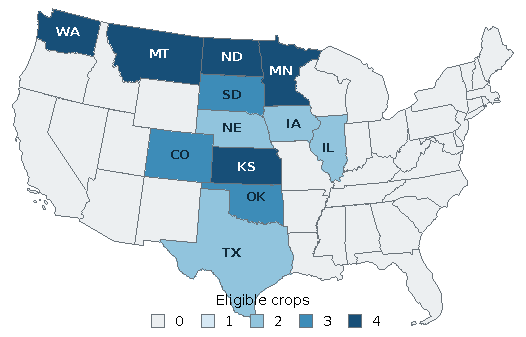
\includegraphics[width=\columnwidth]{locked_crop_state_coverage.pdf}
\caption{Geographic coverage of eligible locked crop--state series. Shading
reports the number of crops represented in each state; coverage is computed
directly from the locked outer-fold row manifest.}
\label{fig:coverage}
\end{figure}

Some early cutoffs did not contain three complete boundary-stage years. Before
any model fitting, the protocol was amended to use medians from a frozen
1981--2025 USDA progress snapshot for those cells. Across the 12 manifests,
calendar definitions comprise 120 frozen crop-season fallbacks, 88 frozen
state fallbacks, 182 cutoff crop-season fallbacks, and 90 cutoff-safe state
definitions. GDD definitions comprise 24 cutoff-safe progress definitions, 24
frozen crop-season fallbacks, and 12 fixed external canola fallbacks. No yield,
validation, or model metric informed this amendment. It nevertheless introduces
retrospective external-source information and is a limitation, not a claim of
prospective deployability.

\section{Factorial Evaluation Protocol}
\subsection{Design and temporal separation}
The design crosses four representations, FLAT versus HIER-RESIDUAL treatment,
COMPACT versus EXPANDED hyperparameter grids, five estimators, and metadata-only,
weather-only, and full feature families. HIER-RESIDUAL uses ridge partial
pooling over crop, state, crop--state intercepts, and centered crop--state time
slopes; unseen groups receive the population-level prediction. The model set is
linear shrinkage, Extra Trees, LightGBM, CatBoost, and histogram gradient
boosting. Table~\ref{tab:design} summarizes the representation arms.

\begin{table}[!t]
\caption{Weather representation component of the 16-arm design.}
\label{tab:design}
\centering\small
\resizebox{\columnwidth}{!}{\begin{tabular}{lrrl}
\toprule
Representation & Arms & Weather vars. & Role \\
\midrule
BASE & 4 & 35 full-season & Reference \\
STAGE-CAL & 4 & 15 calendar-stage & Fixed progress dates \\
STAGE-GDD & 4 & 15 GDD-stage & Heat accumulation \\
STAGE-HYBRID & 4 & 65 combined & BASE + CAL + GDD \\
\bottomrule
\end{tabular}
}
\end{table}

Six expanding outer folds test 2008--2011, 2012--2014, 2015--2017,
2018--2020, 2021--2023, and 2024--2025. Each outer training set contains three
rolling inner folds. Hyperparameters minimize mean inner RMSE, with worst-fold
RMSE and complexity as tie-breakers. Five fixed seeds quantify stochastic model
variation. All preprocessing, trends, hierarchy terms, feature definitions, and
selection are fit without outer-test outcomes.

The complete matrix contains 16 arms, 80 arm--model cells, and 240
feature-family pipelines. Completion was required before leaderboard creation:
34,560 of 34,560 inner jobs and 4,896 of 4,896 seeded outer fits finished.
Across the complete leaderboard, \ExtPassRone\ pipelines pass R1 and
\ExtPassA\ pass Module A. Among 80 full pipelines, \ExtPassB\ pass B and
\ExtPassAB\ pass A+B; \ExtPassE\ E-evaluated candidates pass E.

\subsection{Eligibility modules}
For locked rows, define paired RMSE difference
\begin{equation}
\Delta(a,b)=\operatorname{RMSE}(a)-\operatorname{RMSE}(b).
\end{equation}
Module A compares a candidate against the zero-residual baseline. Module B
compares the full model against the same arm and estimator using metadata only.
Each passes when the upper endpoint of a 2,000-draw calendar-year bootstrap
95\% CI for $\Delta$ is below zero. A crop--state bootstrap is retained as a
sensitivity check.

Module E is evaluated only after A and B pass. Event rows have training-scaled
residual $z<-1$. E requires four conditions: upper 95\% CI below zero for tail
RMSE and MAE differences against zero, positive Spearman rank association with
bootstrap lower endpoint above zero and permutation $p<0.05$, and top-10 lift
above one with bootstrap lower endpoint above one plus hypergeometric and
within-year permutation $p<0.05$. All conditions must pass.

\subsection{Winner lock and external suites}
Eligible pipelines first pass integrity and stable-performance rule R1: pooled
$R^2>0$ and positive fold $R^2$ in at least four of six outer folds. Ranking
then prioritizes claim tier (A+B+E, A+B, A, none), pooled RMSE, worst-fold RMSE,
and complexity, with 0.001 RMSE tie tolerance. The winner and two runners-up
were locked before either external suite was run. Because the winner was
selected from the completed outer-fold leaderboard, its module intervals are
post-selection developmental evidence rather than independent confirmatory
intervals. Confirmation requires a prospectively locked new-year or
external-region holdout.

EXT-SEMI perturbs the four locked candidates across five signal levels, four
measurement-error levels, four spatial-mismatch levels, three event prevalence
levels, and 30 seeds. Its ground-truth labels score permission decisions and
are never model or policy inputs. EXT-PJM uses hourly electricity demand from
EIA-930 \cite{EIA930}; 600 seed-level runs degrade weather by permutation mix,
noise, dropout, or lag substitution. It is cross-domain calibration only and
cannot influence crop selection.

\section{Results}
\subsection{Locked winner and fold stability}
The winner is C310/CatBoost/full: STAGE-HYBRID, HIER-RESIDUAL, and COMPACT.
It produces \ExtRows\ pooled outer predictions with RMSE \ExtRMSE\ t
ha$^{-1}$, MAE \ExtMAE\ t ha$^{-1}$, and $R^2=\ExtRtwo$. The selected
pipeline has positive $R^2$ in \ExtPositiveFolds/6 folds. C300 differs only by
the FLAT treatment and is numerically tied within tolerance; C301 replaces
CatBoost with Extra Trees and is slightly worse (Table~\ref{tab:rank}). The
winner is determined by the locked hierarchy of rules, not by a claim that its
point RMSE is uniquely superior.

\begin{table}[!t]
\caption{Locked ranking after complete factorial evaluation.}
\label{tab:rank}
\centering\scriptsize
\resizebox{\columnwidth}{!}{\begin{tabular}{clllrrrr}
\toprule
Rank & Arm & Model & Family & RMSE & $R^2$ & $R^2{>}0$ & Tier \\
\midrule
1 & C310 & catboost & full & 0.461 & 0.110 & 4/6 & A+B \\
2 & C300 & catboost & full & 0.461 & 0.110 & 4/6 & A+B \\
3 & C301 & extra\_trees & full & 0.462 & 0.106 & 4/6 & A+B \\
\midrule\multicolumn{8}{l}{Candidate-wide passes: R1 38/240; A 122/240; B 46/80 full;} \\
\multicolumn{8}{l}{A+B 46/80 full; E 0/46 evaluated.} \\
\bottomrule
\end{tabular}
}
\end{table}

\begin{figure}[!t]
\centering
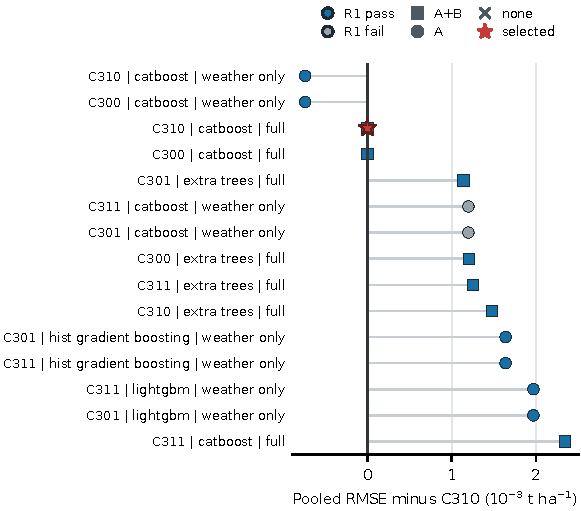
\includegraphics[width=\columnwidth]{leaderboard_delta_rmse.pdf}
\caption{Fifteen lowest-RMSE pipelines, shown as pooled RMSE difference from
C310 on an expanded axis. Blue/gray denote R1 pass/fail; square, circle, and
cross denote A+B, A, and none. The star marks the tier-first selection, which
does not use external-suite results.}
\label{fig:core}
\end{figure}

Table~\ref{tab:folds} shows temporal heterogeneity. Performance is positive in
O1--O4, nearly null in O5, and negative in O6. Pooled adequacy therefore should
not be read as uniformly strong performance through time. The worst-fold RMSE
is 0.610 t ha$^{-1}$, and the final fold $R^2$ is $-0.218$.

\begin{table}[!t]
\caption{Outer-fold performance of locked C310/CatBoost/full.}
\label{tab:folds}
\centering\small
\begin{tabular}{lrrrr}
\toprule
Fold & Test years & RMSE & MAE & $R^2$ \\
\midrule
O1 & 2008--11 & 0.416 & 0.329 & 0.111 \\
O2 & 2012--14 & 0.361 & 0.294 & 0.112 \\
O3 & 2015--17 & 0.468 & 0.357 & 0.050 \\
O4 & 2018--20 & 0.408 & 0.328 & 0.036 \\
O5 & 2021--23 & 0.610 & 0.470 & -0.002 \\
O6 & 2024--25 & 0.485 & 0.366 & -0.218 \\
Pooled & 2008--25 & 0.461 & 0.355 & 0.110 \\
\bottomrule
\end{tabular}

\end{table}

\subsection{Claim-eligibility decision}
Modules A and B both pass. Their paired RMSE difference is
$\ExtGateADelta$ t ha$^{-1}$ with calendar-year bootstrap 95\% CI
[$\ExtGateALow$, $\ExtGateAHigh$]. The equality of A and B to displayed
precision reflects the locked comparator predictions in this arm; it is not a
shared test. Crop--state sensitivity upper endpoints are also negative
($-0.0139$ for each comparison).

Module E fails despite three favorable components. Among \ExtEventRows\ event
rows, tail RMSE difference is \ExtTailRMSEDelta\ t ha$^{-1}$ (95\% CI
[\ExtTailRMSELow, \ExtTailRMSEHigh]) and tail MAE difference is
\ExtTailMAEDelta\ t ha$^{-1}$ (95\% CI [\ExtTailMAELow,
\ExtTailMAEHigh]). Spearman $\rho=0.287$ (bootstrap lower endpoint 0.123;
permutation $p=0.0141$). However, the predicted and observed top-10 sets overlap
in only one row: lift 1.36, bootstrap lower endpoint 0, hypergeometric
$p=0.547$, and within-year permutation $p=0.492$. Because E is conjunctive,
top-$k$ failure blocks event recovery. Table~\ref{tab:modules} records the
paired error components.

\begin{table}[!t]
\caption{Locked paired error statistics. Error differences are in t
ha$^{-1}$; Module E uses $n=136$ event rows.}
\label{tab:modules}
\centering\small
\resizebox{\columnwidth}{!}{\begin{tabular}{llrrr}
\toprule
Module & Comparison & Estimate & 95\% low & 95\% high \\
\midrule
A & Full $-$ zero & -0.028 & -0.045 & -0.013 \\
B & Full $-$ metadata & -0.028 & -0.045 & -0.013 \\
E & Tail RMSE & -0.069 & -0.102 & -0.033 \\
E & Tail MAE & -0.076 & -0.110 & -0.042 \\
\bottomrule
\end{tabular}
}
\end{table}

The resulting tier is A+B. It permits the statement that weather variables add
predictive value to an overall adequate model in this retrospective population.
It does not permit statements that the pipeline recovers particular low-yield
events, that its feature attributions explain observed losses, or that weather
caused those losses. The intervals quantify the selected developmental result;
they do not independently confirm the winner after tier-first selection.

\FloatBarrier
\section{External Calibration}
\subsection{Semi-synthetic permission power}
EXT-SEMI contains \ExtSemiRows\ scored rows from 9,600 base fits. At base event
prevalence, the locked winner's permission rate rises only from 4.0\% at zero
minimum detectable effect (MDE) to 8.8\% at 1.5 MDE. The strongest runner rises
from 9.8\% to 20.0\% (Table~\ref{tab:semi}). Figure~\ref{fig:semi} shows the
complete signal curve by candidate.

\begin{table}[!t]
\caption{EXT-SEMI A+B+E permission rate at base prevalence.}
\label{tab:semi}
\centering\small
\begin{tabular}{lrrr}
\toprule
Candidate & 0 MDE & 1 MDE & 1.5 MDE \\
\midrule
winner & 4.0\% & 6.5\% & 8.8\% \\
runner\_up\_1 & 4.4\% & 6.0\% & 7.5\% \\
runner\_up\_2 & 9.8\% & 14.4\% & 20.0\% \\
kse\_primary & 3.8\% & 4.6\% & 5.0\% \\
\bottomrule
\end{tabular}

\end{table}

\begin{figure}[!t]
\centering
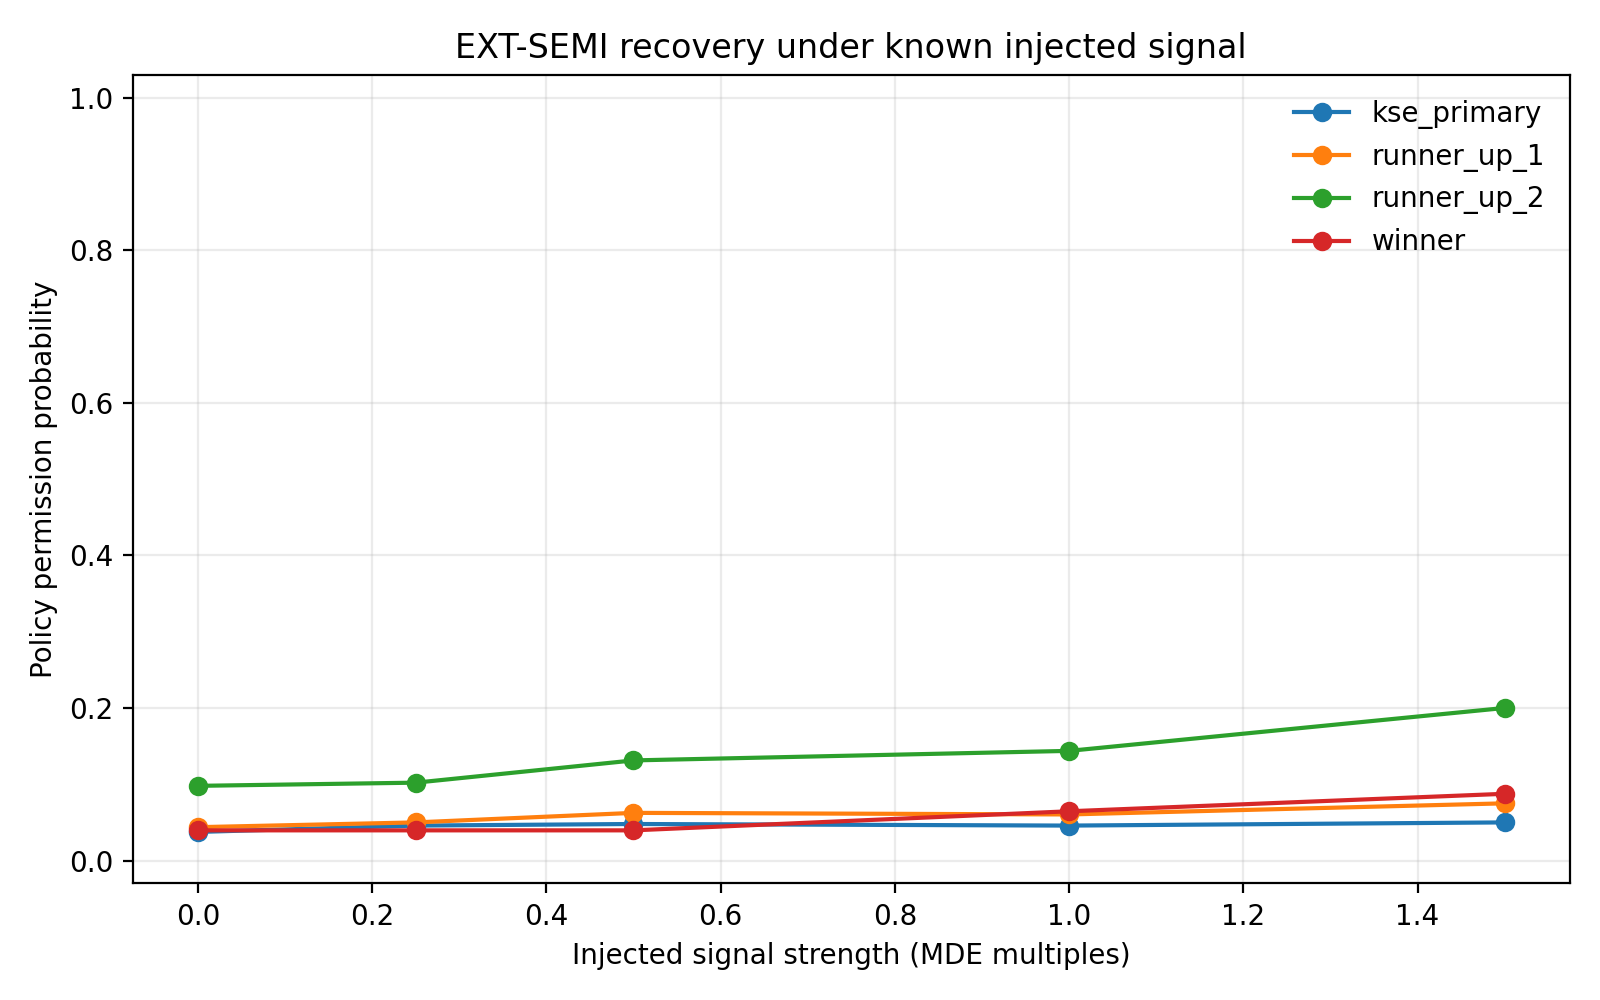
\includegraphics[width=\columnwidth]{semi_permission_power.png}
\caption{Semi-synthetic permission probability versus injected signal at base
event prevalence. Ground-truth labels are evaluation-only; decisions use
observable Modules A, B, and E.}
\label{fig:semi}
\end{figure}

These rates expose high false abstention under the tested data scale and policy.
They should not be reframed as successful event sensitivity. The audit is
conservative, and passing A+B in the crop panel does not resolve the low power
of E.

\subsection{PJM weather degradation}
The PJM suite evaluates whether Module B responds when weather information is
progressively degraded. After common train-median imputation, all
$\lambda=0$ inputs are invariant. At maximum degradation, B-pass probability
is 0 for seven-day lag substitution, 0.50 for two-standard-deviation noise,
0.87 for 75\% dropout, and 0.83 for complete permutation mixing
(Table~\ref{tab:pjm}; Fig.~\ref{fig:pjm}). Thus, B is highly responsive to lag,
partly responsive to additive noise, and comparatively tolerant of the tested
dropout and permutation mechanisms.

\begin{table}[!t]
\caption{EXT-PJM Module-B degradation endpoints.}
\label{tab:pjm}
\centering\small
\resizebox{\columnwidth}{!}{\begin{tabular}{lrrr}
\toprule
Mechanism & Max. level & $P(B)$ at 0 & $P(B)$ at max. \\
\midrule
dropout & 0.75 & 1.00 & 0.87 \\
lag\_substitution & 7 & 1.00 & 0.00 \\
noise & 2 & 1.00 & 0.50 \\
permutation\_mix & 1 & 1.00 & 0.83 \\
\bottomrule
\end{tabular}
}
\end{table}

\begin{figure}[!t]
\centering
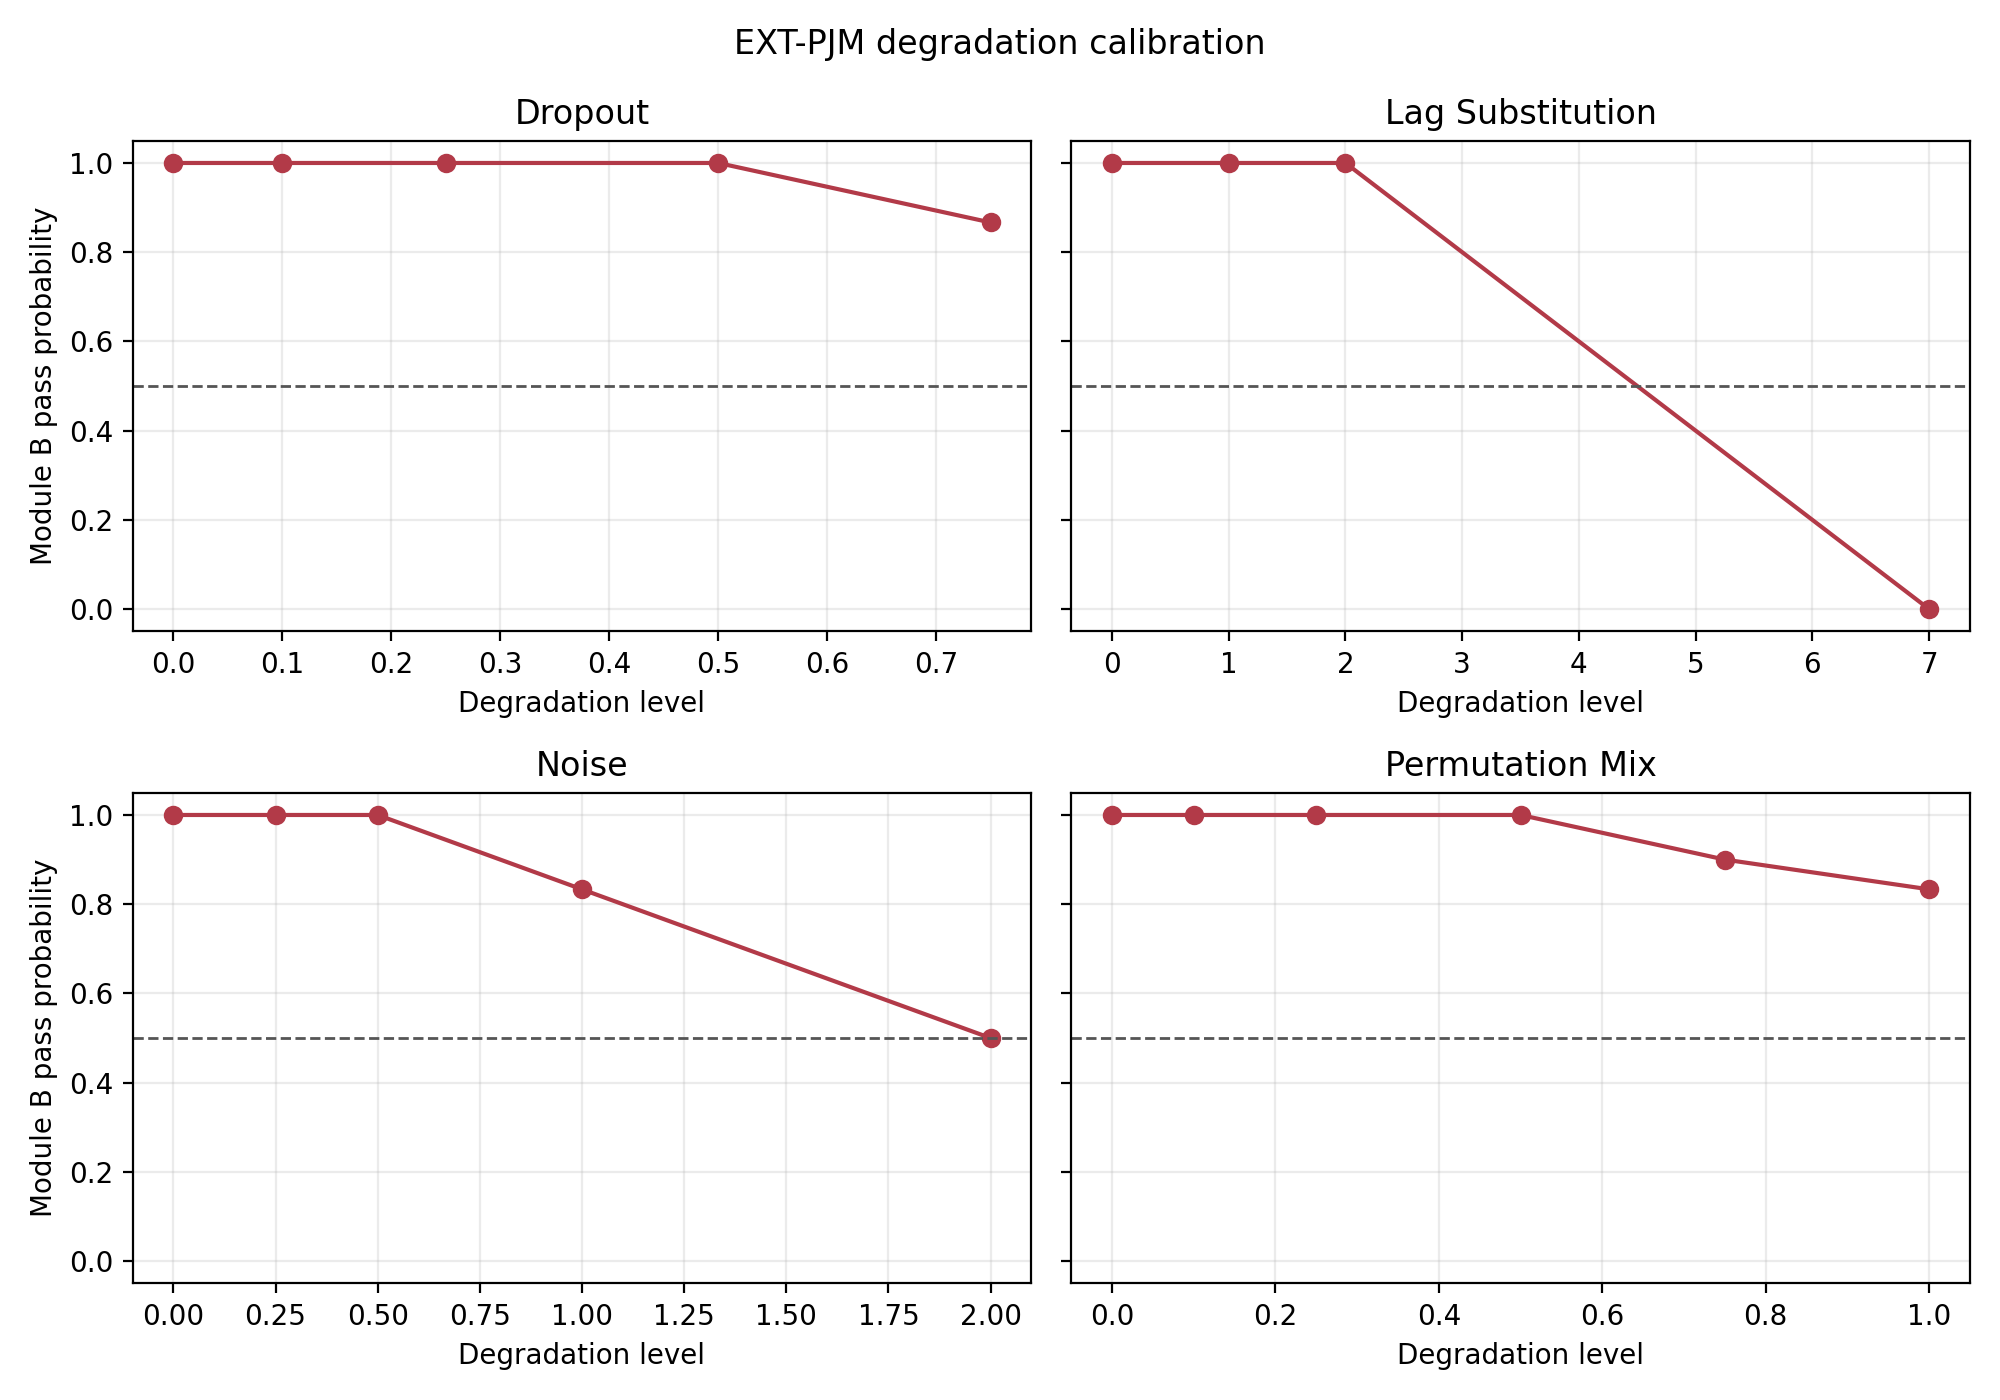
\includegraphics[width=\columnwidth]{pjm_degradation_curves.png}
\caption{Module-B pass probability across 600 PJM degradation runs. Curves are
mechanism-specific calibrations, not crop-model selection evidence.}
\label{fig:pjm}
\end{figure}

This uneven response is informative: a gate that detects one kind of feature
corruption need not detect another. Cross-domain evidence therefore calibrates
behavior but does not validate agricultural transportability.

\FloatBarrier
\section{Discussion}
\subsection{What the factorial study changes}
The factorial result strengthens the developmental basis for an A+B claim in
the evaluated retrospective population relative to a single hand-chosen
pipeline. The locked winner emerges after comparing stage
representations, hierarchy, grid breadth, models, and feature families under
the same temporal protocol. Its nearest competitor is effectively tied, which
argues for a conclusion about the attained claim tier rather than the uniqueness
of C310.

At the same time, the experiment separates three questions that are often
collapsed. Positive pooled skill answers whether useful prediction exists.
Module B asks whether weather adds value beyond metadata. Module E asks whether
the system can identify the specific adverse events that an explanation might
be used to discuss. Here the first two answers are yes and the third is no.
Feature-attribution outputs may therefore describe fitted weather reliance, but
they cannot be presented as explanations of observed event losses.

\subsection{Limitations}
First, 615 locked rows are modest for a five-model factorial comparison, and two
recent folds have non-positive $R^2$. Second, stage definitions partly use a
frozen external crop-progress snapshot where cutoff histories are sparse. This
was declared before fitting and uses no outcomes, but it remains retrospective
information. Third, the semi-synthetic suite shows low A+B+E recovery even as
signal grows; the policy can abstain from valid cases. Fourth, PJM is a useful
mechanism check, not evidence that electricity-demand behavior transfers to
crop yield. Finally, predictive reliance is not causal relevance. Unmeasured
confounding, leakage, and geographic shift can preserve predictive contrasts
\cite{Janzing2020,KapoorNarayanan2023}. Moreover, the tier-first rule was fixed
before execution but does not eliminate selection optimism when the same outer
leaderboard selects and describes the winner. Independent confirmation requires
a prospectively locked new-year or external-region holdout.

Future work should pre-register a prospective stage source, increase event
counts, calibrate thresholds without weakening the event claim, and evaluate
new years and held-out regions. Such studies should retain the rule that
evaluation labels are never policy inputs.

\section{Reproducibility}
The protocol was locked after source-coverage audit and before model fitting.
Checkpointed execution records all 34,560 inner jobs, 4,896 outer fits, 9,600
semi-synthetic base fits, and 600 PJM runs. A completion audit reports 30/30
items complete; the release QA reports 26/26 checks passed, including temporal
access, row integrity, stage manifests, external-suite isolation, seed counts,
and PJM zero-degradation invariance. The run manifest stores package versions,
commands, file hashes, and the winner-lock hash. The frozen earlier manuscript
and PDF are hash-checked and are not modified by this extension.
An anonymized artifact containing the locked manifests, row-level predictions,
completion audit, and figure-generation scripts is available at
\href{https://github.com/Anonymous21223/Claim-Eligibility-Auditing/tree/ictai-v6.1-factorial}
{\nolinkurl{github.com/Anonymous21223/Claim-Eligibility-Auditing/tree/ictai-v6.1-factorial}}.

\section{Conclusion}
A full factorial search does not remove the need to limit explanation claims.
The selected crop-yield pipeline passes overall adequacy and incremental weather
value, but not event recovery. The defensible conclusion is therefore narrow:
weather provides predictive reliance in the evaluated retrospective population,
while explanations remain model-descriptive for individual adverse events.
Semi-synthetic low power and mechanism-dependent PJM degradation further show
that claim eligibility is a transparent scope controller, not a universal
certificate of scientific validity. The result remains post-selection
developmental evidence until tested on a prospectively locked holdout.

\FloatBarrier
\bibliographystyle{IEEEtran}
\bibliography{references_extension}

\end{document}
